\documentclass[11pt]{amsbook}

\usepackage{../HBSuerDemir}

\begin{document}
% ++++++++++++++++++++++++++++++++++++++
\hPage{b2p1/174}
% ++++++++++++++++++++++++++++++++++++++
\begin{exmp}
	\begin{hSolution}
		\footnote{example enumeration continues from the previous page.}
		\begin{hEnumerateAlpha}
			\item Dot product of direction vectors $(1, 0, 3)$ and $(2\lambda + \mu , -3\lambda, -3\mu)$ of the line and the member must vanish:
			\[
				2\lambda + \mu - 9\mu = 0 \Rightarrow \lambda - 4\mu = 0
			\]
			Taking $\lambda = 4$, $\mu = 1$ we have
			\begin{align*}
				4(2x - 3y - 8)+(x - 3z + 8) &= 0 \\
				9x - 12y - 3z - 24 &= 0
			\end{align*}
		\end{hEnumerateAlpha}
	\end{hSolution}
\end{exmp}

\subsection{Intersection, Angle, Distance}
\subsubsection{Intersections}
\begin{enumerate}
	\item \underline{Intersection of a line and a plane:} Let the line $\ell$ and plane $\pi$ be given by the equations.
	\begin{align*}
		\ell &: \frac{x-x_{0}}{a} = \frac{y-y_{0}}{b} = \frac{z-z_{0}}{c} = t \quad &(\vec{D} = (a, b, c)) \\
		\pi &: Ax + By + Cz + D = 0 \quad &(\vec{N} = (A, B, C))
	\end{align*}
	As the relative positions of $\ell$, $\pi$ we have three exhaustive cases:
	\begin{figure}[htbp]
		\begin{center}
			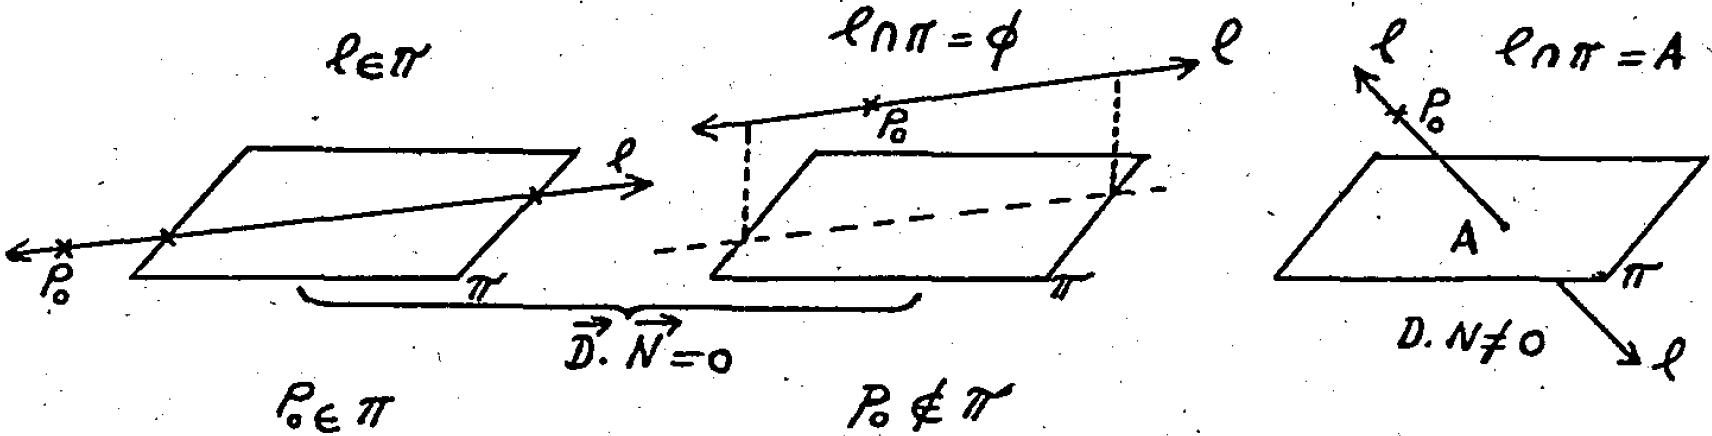
\includegraphics[width=0.8\columnwidth]{images/b2p1-174-fig01.png}
		\end{center}
	\end{figure}
	\par If direction vectors $\vec{D}$ and $\vec{N}$ are perpendicular, one has $\ell\parallel\pi$ in which case either $\ell\in\pi$ or $\ell ? \pi = \emptyset$\footnote{I cannot understand what ? stands for.}. In the first case $P_{0}\in\pi$ and the second $P_{0}\not\in\pi$
	\par If $...$, the line intersects the plane at a point $A$ which is determined by setting the coordinates of any point $P(x_{0} + at, y_{0} + bt, z_{0} + ct)$ of $..$ in the equation of $\pi$, and obtaining a linear equation in $t$. If $t_{1}$ is the solution then $P(t_{1})$ is the required intersection point.
\end{enumerate}
\end{document}